%%%%%%%%%%%%%%%%%%%%%%%%%%%%%%%%%%%%%%%%%%%%%%%%%%%%%%%%%%%%%%%%%%%%%%
\section{サンプル}
\label{sec:sample}

%%%%%%%%%%%%%%%%%%%%%%%%%%%%%%%%%%%%%%%%%%%%%%
\subsection{重力$N$体計算}

\subsubsection{計算1}

以下は様々な多重局展開を使って計算を行った場合の結果である。

{\bf 初期条件}

N=16384、プラマーモデル、非等質量。質量の範囲は一番重い粒子の質量が一
番軽いものの3倍。計算機はcore-i5。並列化は4プロセス*2スレッド。モーメ
ントの計算を、重心展開の単極子と四重極子、さらに幾何中心展開の単極子、
双極子、四重極子まで使った、5つの計算を行った。ツリーのオープニングク
ライテリオンは0.5。最大のi粒子グループ数は64。最大のリーフ粒子数は8。
PhantomGRAPEは使用していない。

{\bf 結果}

\begin{figure}
  \begin{center}
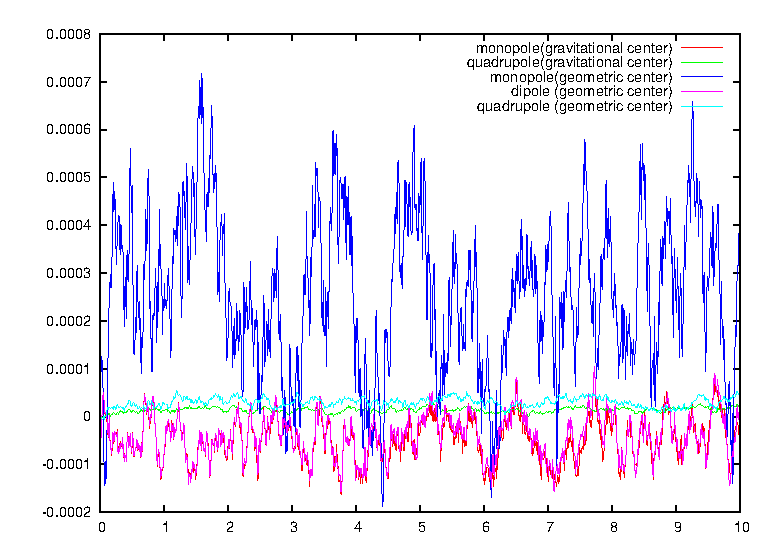
\includegraphics[width=10cm]{fig/relative_energy_error_various_center.eps}
  \end{center}
  \caption{相対エネルギー誤差}
  \label{fig:relative_energy_error_various_center}
\end{figure}

\subsubsection{計算2}

以下は本サンプルコードの計算時間である。

{\bf 初期条件}

N=8M(M=$2^{20}$)のプラマーモデル。粒子はすべて等質量。計算機は京。並列
化は64-2048プロセス*8スレッドの。モーメントの計算は、重心展開の単極子
を使った。ツリーのオープニングクライテリオンは0.5。最大のi粒子グループ
数は64。最大のリーフ粒子数は8。PhantomGRAPEは使用していない。

{\bf 結果}

\begin{figure}
  \begin{center}
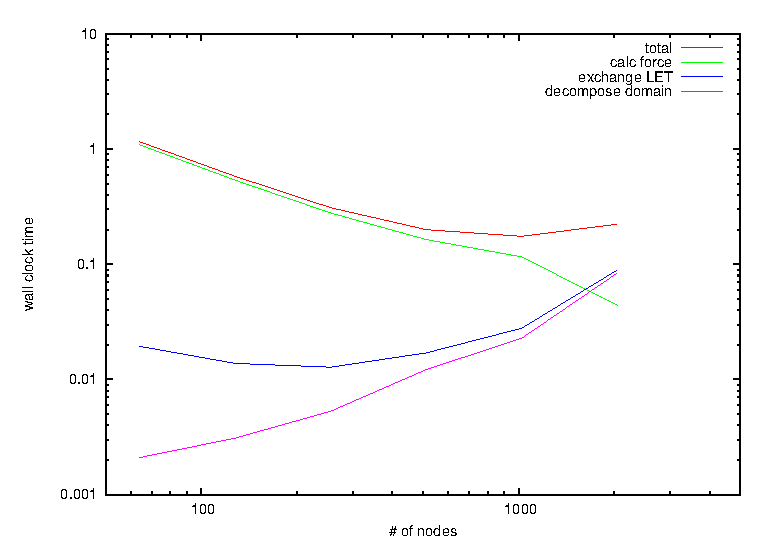
\includegraphics[width=10cm]{fig/nbody_mono_noPHG_tcal.eps}
  \end{center}
  \caption{計算時間}
  \label{fig:nbody_mono_noPHG_tcal}
\end{figure}

\subsubsection{計算3}

以下は本サンプルコードの計算時間である。

{\bf 初期条件}

N=64M(M=$2^{20}$)のプラマーモデル。粒子はすべて等質量。計算機は京。並
列化は512-2048プロセス*8スレッドの。モーメントの計算は、重心展開の単極
子を使った。ツリーのオープニングクライテリオンは0.5。最大のi粒子グルー
プ数は256。最大のリーフ粒子数は8。PhantomGRAPEは使用していない。

{\bf 結果}

\begin{figure}
  \begin{center}
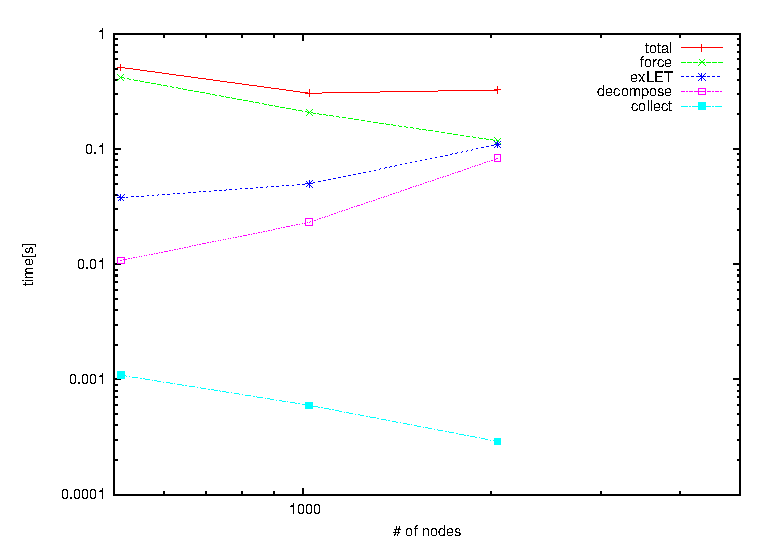
\includegraphics[width=12cm]{fig/nbody_mono_PHG_tcal_N64m.eps}
  \end{center}
  \caption{計算時間}
  \label{fig:nbody_mono_noPHG_tcal}
\end{figure}


\subsubsection{使用コード}


\begin{lstlisting}[caption=重力$N$体計算]
#include<iostream>
#include<fstream>
#include<unistd.h>
#include<particle_simulator.hpp>

#ifdef USEPHANTOMGRAPE
#include"phantomgrape.hpp"
#endif

class ForceGrav{
public:
    PS::F64vec acc;
    PS::F64 pot;
    void clear(){
        acc = 0.0;
        pot = 0.0;
    }
};

class FPGrav{
public:
    PS::S64 id;
    PS::F64 mass;
    PS::F64vec pos;
    PS::F64vec vel;
    PS::F64vec acc;
    PS::F64 pot;
    PS::F64vec getPos() const { return pos; }
    void copyFromForce(const ForceGrav & force){
        acc = force.acc;
        pot = force.pot;
    }
};

class EPIGrav{
public:
    PS::S64 id;
    PS::F64vec pos;
    static PS::F64 eps;
    PS::F64vec getPos() const { return pos;}
    void copyFromFP(const FPGrav & fp){
        pos = fp.pos;
        id = fp.id;
    }
};

PS::F64 EPIGrav::eps = 1.0/32.0;

class EPJGrav{
public:
    PS::S64 id;
    PS::F64 mass;
    PS::F64vec pos;
    void copyFromFP(const FPGrav & fp){
        mass = fp.mass;
        pos = fp.pos;
        id = fp.id;
    }
    PS::F64vec getPos() const { return pos; }
    void setPos(const PS::F64vec & pos_new){ pos = pos_new;}
    PS::F64 getCharge() const { return mass; }
};

#ifdef USEPHANTOMGRAPE

struct CalcForceEpEp{
    void operator () (const EPIGrav * ep_i,
                      const PS::S32 n_ip,
                      const EPJGrav * ep_j,
                      const PS::S32 n_jp,
                      ForceGrav * force){
        double xi[PhantomGRAPE::PG_NIMAX][3];
        double mxj[PhantomGRAPE::PG_NJMAX][4];
        double ai[PhantomGRAPE::PG_NIMAX][3];
        double pi[PhantomGRAPE::PG_NIMAX];
        const PS::F64 eps2 = EPIGrav::eps * EPIGrav::eps;
        const PS::F64 pot_corr = 1.0 / sqrt(eps2) * ep_j[0].getCharge(); // potential correction
        for(PS::S32 i=0; i<n_ip; i++){
            xi[i][0] = ep_i[i].getPos().x;
            xi[i][1] = ep_i[i].getPos().y;
            xi[i][2] = ep_i[i].getPos().z;

        }
        for(PS::S32 j=0; j<n_jp; j++){
            mxj[j][0] = ep_j[j].getPos().x;
            mxj[j][1] = ep_j[j].getPos().y;
            mxj[j][2] = ep_j[j].getPos().z;
            mxj[j][3] = ep_j[j].getCharge();
        }
        PhantomGRAPE pg;
        pg.set_eps2(eps2);
        pg.set_xj(n_jp, mxj);
        pg.set_xi(n_ip, xi);
        pg.run(n_ip, n_jp);
        pg.get_ai(n_ip, ai, pi);

        for(PS::S32 i=0; i<n_ip; i++){
            force[i].acc.x += ai[i][0];
            force[i].acc.y += ai[i][1];
            force[i].acc.z += ai[i][2];
            force[i].pot += pi[i] + pot_corr;
        }
    }
};

#else
struct CalcForceEpEp{
    void operator () (const EPIGrav * ep_i,
                      const PS::S32 n_ip,
                      const EPJGrav * ep_j,
                      const PS::S32 n_jp,
                      ForceGrav * force){

        PS::F64 eps2 = EPIGrav::eps * EPIGrav::eps;
        for(PS::S32 i=0; i<n_ip; i++){
            PS::F64vec xi = ep_i[i].pos;
            PS::F64vec ai = 0.0;
            PS::F64 poti = 0.0;
            PS::S64 idi = ep_i[i].id;
            for(PS::S32 j=0; j<n_jp; j++){
                if( idi == ep_j[j].id ) continue;
                PS::F64vec rij = xi - ep_j[j].pos;
                PS::F64 r3_inv = rij * rij + eps2;
                PS::F64 r_inv = 1.0/sqrt(r3_inv);
                r3_inv = r_inv * r_inv;
                r_inv *= ep_j[j].mass;
                r3_inv *= r_inv;
                ai -= r3_inv * rij;
                poti -= r_inv;
            }
            force[i].acc += ai;
            force[i].pot += poti;
        }
    }
};
#endif // USEPHANTOMGRAPE

#ifdef MONOPOLE

#ifdef USEPHANTOMGRAPE
struct CalcForceSpEp{
    void operator () (const EPIGrav * ep_i,
                      const PS::S32 n_ip,
                      const PS::SPJMonopole * sp_j,
                      const PS::S32 n_jp,
                      ForceGrav * force){
        double xi[PhantomGRAPE::PG_NIMAX][3];
        double mxj[PhantomGRAPE::PG_NJMAX][4];
        double ai[PhantomGRAPE::PG_NIMAX][3];
        double pi[PhantomGRAPE::PG_NIMAX];
        const PS::F64 eps2 = EPIGrav::eps * EPIGrav::eps;
        for(PS::S32 i=0; i<n_ip; i++){
            xi[i][0] = ep_i[i].pos.x;
            xi[i][1] = ep_i[i].pos.y;
            xi[i][2] = ep_i[i].pos.z;
        }
        for(PS::S32 j=0; j<n_jp; j++){
            mxj[j][0] = sp_j[j].getPos().x;
            mxj[j][1] = sp_j[j].getPos().y;
            mxj[j][2] = sp_j[j].getPos().z;
            mxj[j][3] = sp_j[j].getCharge();
        }
        PhantomGRAPE pg;
        pg.set_eps2(eps2);
        pg.set_xj(n_jp, mxj);
        pg.set_xi(n_ip, xi);
        pg.run(n_ip, n_jp);
        pg.get_ai(n_ip, ai, pi);

        for(PS::S32 i=0; i<n_ip; i++){
            force[i].acc.x += ai[i][0];
            force[i].acc.y += ai[i][1];
            force[i].acc.z += ai[i][2];
            force[i].pot += pi[i];
        }

    }
};
#else
struct CalcForceSpEp{
    void operator () (const EPIGrav * ep_i,
                      const PS::S32 n_ip,
                      const PS::SPJMonopole * sp_j,
                      const PS::S32 n_jp,
                      ForceGrav * force){
        PS::F64 eps2 = EPIGrav::eps * EPIGrav::eps;
        for(PS::S32 i=0; i<n_ip; i++){
            PS::F64vec xi = ep_i[i].pos;
            PS::F64vec ai = 0.0;
            PS::F64 poti = 0.0;
            for(PS::S32 j=0; j<n_jp; j++){
                PS::F64vec rij = xi - sp_j[j].pos;
                PS::F64 r3_inv = rij * rij + eps2;
                PS::F64 r_inv = 1.0/sqrt(r3_inv);
                r3_inv = r_inv * r_inv;
                r_inv *= sp_j[j].mass;
                r3_inv *= r_inv;
                ai -= r3_inv * rij;
                poti -= r_inv;
            }
            force[i].acc += ai;
            force[i].pot += poti;
        }
    }
};
#endif // #ifdef USEPHANTOMGRAPE

#elif QUADRUPOLE
struct CalcForceSpEp{
    void operator () (const EPIGrav * ep_i,
                      const PS::S32 n_ip,
                      const PS::SPJQuadrupole * sp_j,
                      const PS::S32 n_jp,
                      ForceGrav * force){
        PS::F64 eps2 = EPIGrav::eps * EPIGrav::eps;
        for(PS::S32 ip=0; ip<n_ip; ip++){
            PS::F64vec xi = ep_i[ip].pos;
            PS::F64vec ai = 0.0;
            PS::F64 poti = 0.0;
            for(PS::S32 jp=0; jp<n_jp; jp++){
                PS::F64 mj = sp_j[jp].mass;
                PS::F64vec xj= sp_j[jp].pos;
                PS::F64vec rij= xi - xj;
                PS::F64 r2 = rij * rij + eps2;
                PS::F64mat qj = sp_j[jp].quad;
                PS::F64 tr = qj.getTrace();
                PS::F64vec qr( (qj.xx*rij.x + qj.xy*rij.y + qj.xz*rij.z),
                               (qj.yy*rij.y + qj.yz*rij.z + qj.xy*rij.x),
                               (qj.zz*rij.z + qj.xz*rij.x + qj.yz*rij.y) );
                PS::F64 qrr = qr * rij;
                PS::F64 r_inv = 1.0f/sqrt(r2);
                PS::F64 r2_inv = r_inv * r_inv;
                PS::F64 r3_inv = r2_inv * r_inv;
                PS::F64 r5_inv = r2_inv * r3_inv * 1.5;
                PS::F64 qrr_r5 = r5_inv * qrr;
                PS::F64 qrr_r7 = r2_inv * qrr_r5;
                PS::F64 A = mj*r3_inv - tr*r5_inv + 5*qrr_r7;
                PS::F64 B = -2.0*r5_inv;
                ai -= A*rij + B*qr;
                poti -= mj*r_inv - 0.5*tr*r3_inv + qrr_r5;
            }
            force[ip].acc += ai;
            force[ip].pot += poti;
        }
    }
};
#elif MONOPOLEGEOMETRICCENTER
struct CalcForceSpEp{
    void operator () (const EPIGrav * ep_i,
                      const PS::S32 n_ip,
                      const PS::SPJMonopoleGeometricCenter * sp_j,
                      const PS::S32 n_jp,
                      ForceGrav * force){
        PS::F64 eps2 = EPIGrav::eps * EPIGrav::eps;
        for(PS::S32 i=0; i<n_ip; i++){
            PS::F64vec xi = ep_i[i].pos;
            PS::F64vec ai = 0.0;
            PS::F64 poti = 0.0;
            for(PS::S32 j=0; j<n_jp; j++){
                PS::F64vec rij = xi - sp_j[j].pos;
                PS::F64 r3_inv = rij * rij + eps2;
                PS::F64 r_inv = 1.0/sqrt(r3_inv);
                r3_inv = r_inv * r_inv;
                r_inv *= sp_j[j].charge;
                r3_inv *= r_inv;
                ai -= r3_inv * rij;
                poti -= r_inv;
            }
            force[i].acc += ai;
            force[i].pot += poti;
        }
    }
};
#elif DIPOLEGEOMETRICCENTER
struct CalcForceSpEp{
    void operator () (const EPIGrav * ep_i,
                      const PS::S32 n_ip,
                      const PS::SPJDipoleGeometricCenter * sp_j,
                      const PS::S32 n_jp,
                      ForceGrav * force){
        const PS::F64 eps2 = EPIGrav::eps * EPIGrav::eps;
        for(PS::S32 i=0; i<n_ip; i++){
            const PS::F64vec xi = ep_i[i].pos;
            PS::F64vec ai = 0.0;
            PS::F64 poti = 0.0;
            for(PS::S32 j=0; j<n_jp; j++){
                const PS::F64vec di = sp_j[j].dipole;
                const PS::F64vec rij = xi - sp_j[j].pos;
                const PS::F64 r2 = rij * rij + eps2;
                const PS::F64 r_inv = 1.0/sqrt(r2);
                const PS::F64 r2_inv = r_inv * r_inv;
                const PS::F64 r3_inv = r_inv * r2_inv;
                const PS::F64vec hij = rij * r_inv;
                const PS::F64 dihij = di * hij;
                const PS::F64 mj = sp_j[j].charge;
                poti -= mj * r_inv + dihij* r2_inv;
                ai -= (mj*r2_inv + 3.0*dihij*r3_inv) * hij - di;
            }
            force[i].acc += ai;
            force[i].pot += poti;
        }
    }
};
#elif QUADRUPOLEGEOMETRICCENTER
struct CalcForceSpEp{
    void operator () (const EPIGrav * ep_i,
                      const PS::S32 n_ip,
                      const PS::SPJQuadrupoleGeometricCenter * sp_j,
                      const PS::S32 n_jp,
                      ForceGrav * force){
        const PS::F64 eps2 = EPIGrav::eps * EPIGrav::eps;
        for(PS::S32 ip=0; ip<n_ip; ip++){
            const PS::F64vec xi = ep_i[ip].pos;
            PS::F64vec ai = 0.0;
            PS::F64 poti = 0.0;
            for(PS::S32 jp=0; jp<n_jp; jp++){
                PS::F64 mj = sp_j[jp].charge;
                PS::F64vec xj= sp_j[jp].pos;
                PS::F64vec rij= xi - xj;
                PS::F64 r2 = rij * rij + eps2;
                PS::F64mat qj = sp_j[jp].quadrupole;
                PS::F64 tr = qj.getTrace();
                PS::F64vec qr( (qj.xx*rij.x + qj.xy*rij.y + qj.xz*rij.z),
                               (qj.yy*rij.y + qj.yz*rij.z + qj.xy*rij.x),
                               (qj.zz*rij.z + qj.xz*rij.x + qj.yz*rij.y) );
                PS::F64 qrr = qr * rij;
                PS::F64 r_inv = 1.0f/sqrt(r2);
                PS::F64 r2_inv = r_inv * r_inv;
                PS::F64 r3_inv = r2_inv * r_inv;
                PS::F64 r5_inv = r2_inv * r3_inv * 1.5;
                PS::F64 qrr_r5 = r5_inv * qrr;
                PS::F64 qrr_r7 = r2_inv * qrr_r5;
                PS::F64 A = mj*r3_inv - tr*r5_inv + 5*qrr_r7;
                PS::F64 B = -2.0*r5_inv;
                ai -= A*rij + B*qr;
                poti -= mj*r_inv - 0.5*tr*r3_inv + qrr_r5;
                const PS::F64vec di = sp_j[jp].dipole;
                const PS::F64 dirij = di * rij;
                poti -= dirij* r3_inv;
                ai -= 3.0*dirij*r5_inv*rij - di;
            }
            force[ip].acc += ai;
            force[ip].pot += poti;
        }
    }
};
#endif

template<class Tpsys>
void ReadNemoAscii(Tpsys & psys,
                   PS::S32 & n_glb,
                   PS::S32 & n_loc,
                   PS::F32 & t_sys,
                   const char * ifile){
    std::ifstream finput;
    finput.open(ifile);
    assert(finput);
    PS::S32 dim;
    finput>>n_glb>>dim>>t_sys;
    std::cerr<<"ifile:"<<ifile<<std::endl;
    std::cerr<<"n_glb="<<n_glb<<std::endl;
    std::cerr<<"dim="<<dim<<std::endl;
    std::cerr<<"t_sys="<<t_sys<<std::endl;

    PS::S32 my_rank = PS::Comm::getRank();
    PS::S32 n_proc = PS::Comm::getNumberOfProc();
    n_loc = n_glb/n_proc;
    if( n_glb % n_proc > my_rank) n_loc++;

    psys.createParticle((n_glb/n_proc)*8+10000);
    psys.setNumberOfParticleLocal(n_loc);

    PS::F32vec pos_shift = 0.0;

    PS::S32 i_h = n_glb/n_proc*my_rank;
    if( n_glb % n_proc  > my_rank) i_h += my_rank;
    else i_h += n_glb % n_proc;
    const PS::S32 i_t = i_h+n_loc;
    PS::F32 xf32;
    PS::F32vec vf32;

    for(PS::S32 i=i_h, n=0; i<i_t; i++, n++)psys[n].id = i;

    for(PS::S32 i=0; i<i_h; i++) finput>>xf32;
    for(PS::S32 i=i_h, n=0; i<i_t; i++, n++){
        finput>>psys[n].mass;
        //psys[n].mass *= (PS::MT::genrand_real1()+0.5);
    }
    for(PS::S32 i=i_t; i<n_glb; i++) finput>>xf32;

    for(PS::S32 i=0; i<i_h; i++) finput>>vf32;
    for(PS::S32 i=i_h, n=0; i<i_t; i++, n++){
        finput>>psys[n].pos;
        psys[n].pos += pos_shift;
    }
    for(PS::S32 i=i_t; i<n_glb; i++) finput>>vf32;

    for(PS::S32 i=0; i<i_h; i++) finput>>vf32;
    for(PS::S32 i=i_h, n=0; i<i_t; i++, n++) finput>>psys[n].vel;
    for(PS::S32 i=i_t; i<n_glb; i++) finput>>vf32;
    finput.close();
}

template<class Tpsys>
void WriteNemoAscii(const Tpsys & psys,
                    const PS::F32 time_sys,
                    const PS::S32 snp_id,
                    const char * dir_name){
    const PS::S32 n_loc = psys.getNumberOfParticleLocal();
    PS::S32 n_glb = 0;
    FPGrav * fp;
    PS::AllGatherParticle(fp, n_glb, &psys[0], n_loc);
    if(PS::Comm::getRank () == 0){
        const PS::S32 STRINGSIZE = 1024;
        char sout[STRINGSIZE];
        sprintf(sout,"%s/snap%5d.dat", dir_name, snp_id);
        for(int i=0;i<STRINGSIZE;i++)if(sout[i]==' ')sout[i]='0';
        std::ofstream foutput;
        foutput.open(sout);
        foutput<<std::setprecision(15);
        foutput<<n_glb<<std::endl;
        foutput<<"3"<<std::endl;
        foutput<<time_sys<<std::endl;
        for(PS::S32 i=0; i<n_glb; i++) foutput<<fp[i].mass<<std::endl;
        for(PS::S32 i=0; i<n_glb; i++) foutput<<fp[i].pos<<std::endl;
        for(PS::S32 i=0; i<n_glb; i++) foutput<<fp[i].vel<<std::endl;
        foutput.close();
    }
}

template<class Tpsys>
void Kick(Tpsys & system,
          const PS::F64 dt){
    PS::S32 n = system.getNumberOfParticleLocal();
    for(int i=0; i<n; i++){
        system[i].vel  += system[i].acc * dt;
    }
}

template<class Tpsys>
void Drift(Tpsys & system,
           const PS::F64 dt){
    PS::S32 n = system.getNumberOfParticleLocal();
    for(int i=0; i<n; i++){
        system[i].pos  += system[i].vel * dt;
    }
}

template<class Tpsys>
void CalcEnergy(const Tpsys & system,
                PS::F64 & etot,
                PS::F64 & ekin,
                PS::F64 & epot,
                const bool clear=true){
    if(clear){
        etot = ekin = epot = 0.0;
    }
    PS::F64 etot_loc = 0.0;
    PS::F64 ekin_loc = 0.0;
    PS::F64 epot_loc = 0.0;
    const PS::S32 nbody = system.getNumberOfParticleLocal();
    for(PS::S32 i=0; i<nbody; i++){
        ekin_loc += system[i].mass * system[i].vel * system[i].vel;
        epot_loc += system[i].mass * system[i].pot;
    }
    ekin_loc *= 0.5;
    epot_loc *= 0.5;
    etot_loc = ekin_loc + epot_loc;
    MPI::COMM_WORLD.Allreduce(&etot_loc, &etot, 1, PS::GetDataType<PS::F64>(), MPI::SUM);
    MPI::COMM_WORLD.Allreduce(&epot_loc, &epot, 1, PS::GetDataType<PS::F64>(), MPI::SUM);
    MPI::COMM_WORLD.Allreduce(&ekin_loc, &ekin, 1, PS::GetDataType<PS::F64>(), MPI::SUM);
}

int main(int argc, char *argv[]){
    PS::F64 Tbegin = PS::GetWtime();
    std::cout<<std::setprecision(15);
    std::cerr<<std::setprecision(15);
    PS::Initialize(argc, argv);
    PS::F32 theta = 0.5;
    const PS::S32 n_leaf_limit = 8;
    PS::S32 n_group_limit = 64;
    PS::F32 time_end = 10.0;
    char sinput[1024];
    char dir_name[1024];
    int c;
    while((c=getopt(argc,argv,"i:o:t:T:n:h")) != -1){
        switch(c){
        case 'i':
            sprintf(sinput,optarg);
            break;
        case 'o':
            sprintf(dir_name,optarg);
            break;
        case 't':
            theta = atof(optarg);
            std::cerr<<"theta="<<theta<<std::endl;
            break;
        case 'T':
            time_end = atof(optarg);
            std::cerr<<"time_end="<<time_end<<std::endl;
            break;
        case 'n':
            n_group_limit = atoi(optarg);
            std::cerr<<"n_group_limit="<<n_group_limit<<std::endl;
            break;
        case 'h':
            std::cerr<<"i: input file name (nemo ascii)"<<std::endl;
            std::cerr<<"o: dir name of output"<<std::endl;
            std::cerr<<"t: theta (dafult: 0.5)"<<std::endl;
            std::cerr<<"T: time_end (dafult: 10.0)"<<std::endl;
            std::cerr<<"n: n_group_limit (dafult: 64.0)"<<std::endl;
            return 0;
        }
    }

    std::ofstream fout_eng;
    std::ofstream fout_tcal;
    
    char sout_de[1024];
    char sout_tcal[1024];
    sprintf(sout_de, "%s/t-de.dat", dir_name);
    sprintf(sout_tcal, "%s/t-tcal.dat", dir_name);
    std::cerr<<sout_de<<std::endl;
    std::cerr<<sout_tcal<<std::endl;
    fout_eng.open(sout_de);
    fout_tcal.open(sout_tcal);

    PS::ParticleSystem<FPGrav> system_grav;
    system_grav.initialize();
    PS::S32 n_grav_glb, n_grav_loc;
    PS::F32 time_sys;
    ReadNemoAscii(system_grav, n_grav_glb, n_grav_loc, time_sys, sinput);
    const PS::F32 coef_ema = 0.7;
    PS::DomainInfo dinfo;
    dinfo.initialize(coef_ema);
    dinfo.collectSampleParticle(system_grav);
    dinfo.decomposeDomain();
    system_grav.exchangeParticle(dinfo);
    n_grav_loc = system_grav.getNumberOfParticleLocal();
#ifdef MONOPOLE
    PS::TreeForForceLong<ForceGrav, EPIGrav, EPJGrav>::Monopole tree_grav;
#elif QUADRUPOLE
    PS::TreeForForceLong<ForceGrav, EPIGrav, EPJGrav>::Quadrupole tree_grav;
#elif MONOPOLEGEOMETRICCENTER
    PS::TreeForForceLong<ForceGrav, EPIGrav, EPJGrav>::MonopoleGeometricCenter tree_grav;
#elif DIPOLEGEOMETRICCENTER
    PS::TreeForForceLong<ForceGrav, EPIGrav, EPJGrav>::DipoleGeometricCenter tree_grav;
#elif QUADRUPOLEGEOMETRICCENTER
    PS::TreeForForceLong<ForceGrav, EPIGrav, EPJGrav>::QuadrupoleGeometricCenter tree_grav;
#endif

    tree_grav.initialize(n_grav_glb, theta, n_leaf_limit, n_group_limit);

    tree_grav.calcForceAllAndWriteBack(CalcForceEpEp(), CalcForceSpEp(), system_grav, dinfo);
#ifdef CHECKFORCE
    tree_grav.checkForce( CalcForceEpEp(), CompareGrav(), dinfo);
#else

    PS::F64 Epot0, Ekin0, Etot0, Epot1, Ekin1, Etot1;
    CalcEnergy(system_grav, Etot0, Ekin0, Epot0);

    const PS::F32 dt = 1.0/128.0;

    Kick(system_grav, dt*0.5);

    PS::F64 Tloop = 0.0;

    PS::S32 snp_id = 0;
    while(time_sys < time_end){

        PS::Timer timer;
        timer.reset();
        timer.start();
        if( fmod(time_sys, 10.0) == 0.0){
            WriteNemoAscii(system_grav, time_sys, snp_id, dir_name);
            snp_id++;
        }
        timer.restart("WriteNemoAscii");

        time_sys += dt;
        Drift(system_grav, dt);

        timer.restart("Drift");

        if( fmod(time_sys, 1.0/32.0) == 0.0){
            dinfo.collectSampleParticle(system_grav, Tloop);
            dinfo.decomposeDomain();
        }

        timer.restart("collect+decompose");

        system_grav.exchangeParticle(dinfo);

        timer.restart("exchangeParticle");

        Tloop = PS::GetWtime();

        tree_grav.calcForceAllAndWriteBackWithTimer
            (CalcForceEpEp(), CalcForceSpEp(), system_grav, dinfo, timer, true);

        Tloop = PS::GetWtime() - Tloop;


        Kick(system_grav, dt*0.5);

        timer.stop("Kick");

        fout_tcal<<"time_sys= "<<time_sys<<std::endl;
        fout_tcal<<"tree_grav.getMemSizeUsed()= "<<tree_grav.getMemSizeUsed()*1e-9<<" [Gbyte]";
        fout_tcal<<" system_grav.getMemSizeUsed()= "<<system_grav.getMemSizeUsed()*1e-9<<" [Gbyte]"<<std::endl;
        tree_grav.dump_calc_cost(PS::Comm::getMaxValue(Tloop), fout_tcal);
        fout_tcal<<"Tloop= "<<Tloop<<" Ttot="<<PS::GetWtime()-Tbegin<<std::endl;
        timer.dump(fout_tcal);
        fout_tcal<<std::endl;

        CalcEnergy(system_grav, Etot1, Ekin1, Epot1);
        if(PS::Comm::getRank() == 0){
            fout_eng<<time_sys<<"   "<<(Etot1-Etot0)/Etot0<<std::endl;
        }
        Kick(system_grav, dt*0.5);
    }

#endif

    PS::Finalize();
    return 0;
}
\end{lstlisting}



%%%%%%%%%%%%%%%%%%%%%%%%%%%%%%%%%%%%%%%%%%%%%%
\subsection{衝撃波菅問題}

\subsubsection{計算1}

以下では一次元衝撃波菅問題を3次元ツリー構造を使って解く。

{\bf 初期条件}

粒子数は1000で、$0 \le x < 1$に等間隔で分布させる。$(\rho, p,
v_{x})=(1.0, 2.5, 0.0), (0.25, 1.795, 0.0)$。前者が$0 \le x < 0.5$、後
者が$0.5 \le x < 1$の場合。$\alpha=0.9$、$\gamma=1.4$、時間刻みの精度パ
ラメータ$0.1$。

{\bf 結果}

\begin{figure}
  \begin{center}
%%    \includegraphics[width=8cm,angle=270]{fig/x-rho.eps}
  \end{center}
  \caption{密度}
  \label{fig:x-rho}
\end{figure}

\begin{figure}
  \begin{center}
%%    \includegraphics[width=8cm,angle=270]{fig/x-p.eps}
  \end{center}
  \caption{圧力}
  \label{fig:x-p}
\end{figure}

\begin{figure}[h]
  \begin{center}
%%    \includegraphics[width=8cm,angle=270]{fig/x-vx.eps}
  \end{center}
  \caption{速度}
  \label{fig:x-vx}
\end{figure}

\subsubsection{計算2}

以下では粒子をランダムにばら撒いた時の計算である。

{\bf 初期条件}

粒子数は6.4e7で、$0 \le x < 1$にランダムに分布させる。$P=1$、
$\alpha=1.0$、$\gamma=1.4$。

{\bf 結果}

以下は京512-4096ノードで行った場合の1ステップの計算時間である。

\begin{figure}
  \begin{center}
    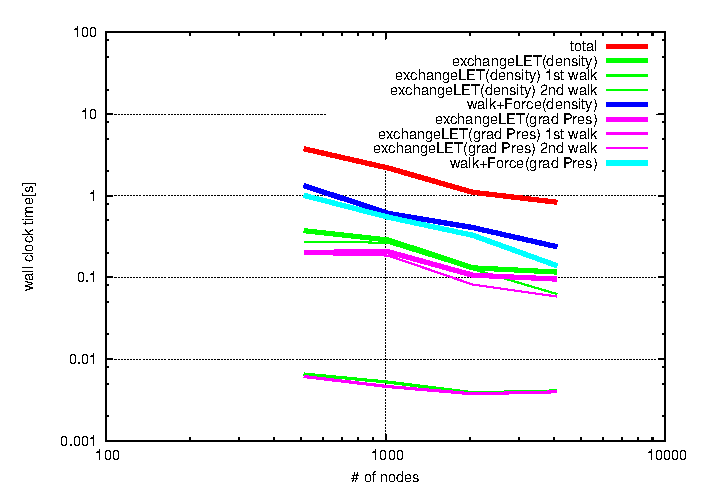
\includegraphics[width=12cm]{fig/tcal_sph_n64M_unirandom.eps}
  \end{center}
  \caption{計算時間}
  \label{fig:tcal_sph_n64M_unirandom}
\end{figure}

{\bf 使用コード}

\begin{lstlisting}[caption=SPHサンプル使用]

#include<iostream>
#include<fstream>
#include<unistd.h>
#include<particle_simulator.hpp>

PS::F64 CubicSpline(const PS::F64 r_sq,
                    const PS::F64 h_inv){
    PS::F64 xi = sqrt(r_sq) * h_inv;
    PS::F64 xi10 = (1.0-xi > 0.0) ? 1.0-xi : 0.0;
    PS::F64 xi05 = (0.5-xi > 0.0) ? 0.5-xi : 0.0;
    return xi10*xi10*xi10 - 4.0*xi05*xi05*xi05;
}

PS::F64vec CubicSpline_ri(const PS::F64vec & rij,
                          const PS::F64 h_inv){
    PS::F64 r_sq = rij * rij;
    PS::F64 r = sqrt(r_sq);
    PS::F64 xi = r * h_inv;
    PS::F64 xi10 = (1.0-xi > 0.0) ? 1.0-xi : 0.0;
    PS::F64 xi05 = (0.5-xi > 0.0) ? 0.5-xi : 0.0;
    PS::F64 C = (3.0*xi10*xi10 - 12.0*xi05*xi05) * h_inv / r;
    return -C * rij;
}

class ResultDens{
public:
    PS::F64 dens;
    PS::F64 divv;
    void clear(){
        dens = divv = 0.0;
    }
};

class ResultForce{
public:
    PS::F64 eng_dot;
    PS::F64vec acc;
    void clear(){
        acc = 0.0;
        eng_dot = 0.0;
    }
};

class FullPtcl{
public:

    PS::F64 getCharge() const {
        return this->mass;
    }
    PS::F64vec getPos() const {
        return this->pos;
    }
    PS::F64 getRSearch() const {
        return this->kernel_length;
    }
    void copyFromForce(const ResultDens & rd){
        dens = rd.dens;
        divv = rd.divv;
    }
    void copyFromForce(const ResultForce & rf){
        acc = rf.acc;
        eng_dot = rf.eng_dot;
    }

    PS::F64 mass;
    PS::F64vec pos;
    PS::F64 kernel_length;
    PS::F64 dens;
    PS::F64 divv;
    PS::F64 pres;
    PS::F64 vel_sound;
    PS::F64vec acc;
    PS::F64 eng_dot;
    PS::S64 id;
    PS::F64vec vel;
    PS::F64 eng;
    PS::F64vec vel_half;
    PS::F64 eng_half;
    PS::S64 n_neighbour;
    void dump(std::ostream & fout=std::cout) const {
        fout<<"pos="<<pos<<std::endl;
        fout<<"dens="<<dens<<std::endl;
        fout<<"kernel_length="<<kernel_length<<std::endl;
    }
};


class EPIDens{
public:
    PS::S64 id;
    PS::F64vec pos;
    PS::F64vec vel;
    PS::F64vec getPos() const { return pos;}
    void copyFromFP(const FullPtcl & fp){
        id = fp.id;
        pos = fp.getPos();
    }
};

class EPJDens{
public:
    PS::S64 id;
    PS::F64 mass;
    static PS::F64 kernel_length;
    PS::F64vec pos;
    PS::F64vec vel;
    PS::F64 getCharge() const { return mass; }
    PS::F64vec getPos() const { return pos; }
    PS::F64 getRSearch() const { return kernel_length; }
    void copyFromFP(const FullPtcl & fp){
        id = fp.id;
        mass = fp.getCharge();
        kernel_length = fp.getRSearch();
        pos = fp.getPos();
    }
};

PS::F64 EPJDens::kernel_length;

struct CalcDensEpEp{
    void operator () (const EPIDens * ep_i,
                      const PS::S32 n_ip,
                      const EPJDens * ep_j,
                      const PS::S32 n_jp,
                      ResultDens * dens){
        static const PS::F64 h_inv = 1.0/ep_j[0].kernel_length;
        static const PS::F64 r_crit_sq = ep_j[0].kernel_length * ep_j[0].kernel_length;
        static const PS::F64 Cnorm = 8.0/3.0 * h_inv; // 1D
        //static PS::F64 Cnorm = 80.0/(7.0*M_PI); // 2D
        //static PS::F64 Cnorm = 16.0/M_PI; // 3D
        for(PS::S32 i=0; i<n_ip; i++){
            dens[i].clear();
            for(PS::S32 j=0; j<n_jp; j++){
                const PS::F64vec rij = ep_i[i].getPos() - ep_j[j].getPos();
                const PS::F64 r_sq = rij * rij;
                if( r_crit_sq > r_sq ){
                    dens[i].dens += ep_j[j].getCharge() * CubicSpline(r_sq, h_inv);
                }
            }
            dens[i].dens *= Cnorm;
            PS::F64 divv = 0.0;
            PS::F64 inv_dens = 1.0/dens[i].dens;
            for(PS::S32 j=0; j<n_jp; j++){
                if(ep_i[i].id == ep_j[j].id) continue;
                const PS::F64vec rij = ep_i[i].getPos() - ep_j[j].getPos();
                const PS::F64vec vij = ep_i[i].vel - ep_j[j].vel;
                const PS::F64 mj = ep_j[j].mass;
                divv -= mj * vij * CubicSpline_ri(rij, h_inv);
            }
            dens[i].divv = divv * Cnorm * inv_dens;
        }
    }
};


template<class Tpsys>
void CalcPressureAndSoundVelocity(Tpsys & system, const PS::F32 gamma){
    const PS::F32 C = gamma - 1.0;
    const PS::S32 n_ptcl = system.getNumberOfParticleLocal();
    for(PS::S32 i=0; i<n_ptcl; i++){
        system[i].pres = C * system[i].dens * system[i].eng;
        system[i].vel_sound = sqrt(gamma * system[i].pres / system[i].dens);
    }
}

class EPIForce{
public:
    PS::F64vec pos;
    PS::F64vec vel;
    PS::F64 divv;
    PS::F64 vel_sound;
    PS::F64 dens;
    PS::F64 pres;
    PS::F64 kernel_length;
    PS::S64 id;
    static PS::F64 alpha;
    void copyFromFP(const FullPtcl & fp){
        pos = fp.pos;
        vel = fp.vel;
        divv = fp.divv;
        vel_sound = fp.vel_sound;
        dens = fp.dens;
        pres = fp.pres;
        kernel_length = fp.kernel_length;
        id = fp.id;
    }
};

PS::F64 EPIForce::alpha = 0.9;

class EPJForce{
public:
    PS::F64vec pos;
    PS::F64vec vel;
    PS::F64 divv;
    PS::F64 vel_sound;
    PS::F64 pres;
    PS::F64 dens;
    PS::F64 kernel_length;
    PS::F64 mass;
    PS::S64 id;
    PS::F64vec getPos() const {return pos;}
    PS::F64 getRSearch() const {return kernel_length;}
    void copyFromFP(const FullPtcl & fp){
        pos = fp.pos;
        vel = fp.vel;
        divv = fp.divv;
        vel_sound = fp.vel_sound;
        pres = fp.pres;
        dens = fp.dens;
        kernel_length = fp.kernel_length;
        mass = fp.mass;
        id = fp.id;
    }
};

struct CalcForceEpEp{
    void operator () (const EPIForce * ep_i,
                      const PS::S32   n_ip,
                      const EPJForce * ep_j,
                      const PS::S32   n_jp,
                      ResultForce    * force){
        for(PS::S32 i=0; i<n_ip; i++){
            PS::F64 cs_i = ep_i[i].vel_sound;
            PS::F64 h_i = ep_i[i].kernel_length;
            PS::F64 inv_h_i = 1.0 / h_i;
            PS::F64 Cnorm_i = (8.0/3.0) * inv_h_i; // 1D
            PS::F64 dens_i = ep_i[i].dens;
            PS::F64 pres_i = ep_i[i].pres;
            PS::F64 f_grad_i = 1.0;
            PS::F64 fp_dens_i = f_grad_i * pres_i / (dens_i * dens_i);
            PS::F64 alpha = EPIForce::alpha;
            PS::F64vec acc = 0.0;
            PS::F64 udot0 = 0.0;
            PS::F64 udot1 = 0.0;
            for(PS::S32 j=0; j<n_jp; j++){
                PS::F64 mj = ep_j[j].mass;
                PS::F64vec r_ij = ep_i[i].pos - ep_j[j].pos;
                if(ep_i[i].id == ep_j[j].id) continue;
                PS::F64vec v_ij = ep_i[i].vel - ep_j[j].vel;
                PS::F64 r_sq = r_ij * r_ij;
                PS::F64 h_j = ep_j[j].kernel_length;
                PS::F64 inv_h_j = 1.0 / h_j;
                PS::F64 Cnorm_j = (8.0/3.0) * inv_h_j; // 1D
                PS::F64 h_ij = (h_i + h_j) * 0.5;
                PS::F64 inv_h_ij = 1.0 / h_ij;
                PS::F64 Cnorm_ij = (8.0/3.0) * inv_h_ij; // 1D
                PS::F64 dens_j = ep_j[j].dens;
                PS::F64 pres_j = ep_j[j].pres;
                PS::F64 f_grad_j = 1.0;
                PS::F64 fp_dens_j = f_grad_j * pres_j / (dens_j * dens_j);
                PS::F64 dens_ij = (dens_i + dens_j) * 0.5;
                PS::F64 w_ij = v_ij * r_ij / sqrt(r_sq);
                PS::F64 vel_sig = cs_i + ep_j[j].vel_sound - 3*w_ij;
                PS::F64 pi_ij = -alpha*0.5*vel_sig*w_ij / dens_ij;
                pi_ij = ( r_ij * v_ij <= 0.0 ) ? pi_ij : 0.0;
                PS::F64vec grad_w_i = Cnorm_i * CubicSpline_ri(r_ij, inv_h_i);
                PS::F64vec grad_w_j = Cnorm_j * CubicSpline_ri(r_ij, inv_h_j);
                PS::F64vec grad_w_ij = Cnorm_ij * CubicSpline_ri(r_ij, inv_h_ij);
                acc -= mj * ( fp_dens_i * grad_w_i + fp_dens_j * grad_w_j
                              + pi_ij * grad_w_ij );
                PS::F64vec mjvij = mj * v_ij;
                udot0 += mjvij * grad_w_i;
                udot1 += pi_ij * mjvij * grad_w_ij;
            }
            force[i].acc = acc;
            force[i].eng_dot = fp_dens_i * udot0 + 0.5 * udot1;
        }
    }
};

template<class Tpsys>
void Kick1( Tpsys & system,
            const PS::F64 dt){
    PS::S32 n = system.getNumberOfParticleLocal();
    for(PS::S32 i=0; i<n; i++){
        system[i].vel_half  = system[i].vel + system[i].acc * dt;
        system[i].eng_half  = system[i].eng + system[i].eng_dot * dt;
    }
}

template<class Tpsys>
void Drift( Tpsys & system,
            const PS::F64 dt){
    PS::S32 n = system.getNumberOfParticleLocal();
    for(PS::S32 i=0; i<n; i++){
        system[i].pos  += system[i].vel_half * dt; // corrected value
        system[i].vel  += system[i].acc * dt;           // predicted value
        system[i].eng  += system[i].eng_dot * dt;        // predicted value
    }
}

template<class Tpsys>
void Kick2( Tpsys & system,
            const PS::F64 dt){
    PS::S32 n = system.getNumberOfParticleLocal();
    for(PS::S32 i=0; i<n; i++){
        system[i].vel  = system[i].vel_half + system[i].acc * dt;
        system[i].eng  = system[i].eng_half + system[i].eng_dot * dt;
    }
}

template<class Tpsys>
PS::F64 CalcDt(Tpsys & system,
               const PS::F64 Ccfl){
    PS::S32 n = system.getNumberOfParticleLocal();
    PS::F64 dt = 99999.9;
    for(PS::S32 i=0; i<n; i++){
        dt = (dt < (system[i].kernel_length/system[i].vel_sound)) ? dt : (system[i].kernel_length/system[i].vel_sound);
    }
    PS::F64 dt_glb = PS::GetMinValue(dt);
    return dt_glb * Ccfl;
}

template<class Tpsys>
void ReadSPHFormat(Tpsys & psys,
                   PS::S32 & n_glb,
                   PS::S32 & n_loc,  
                   PS::F64 & t_sys,
                   const char * ifile){
    std::ifstream finput;
    finput.open(ifile);
    assert(finput);
    PS::S32 dim;
    finput>>n_glb>>dim>>t_sys;

    PS::S32 my_rank = PS::Comm::getRank();
    PS::S32 n_proc = PS::Comm::getNumberOfProc();
    n_loc = n_glb/n_proc; 
    if( n_glb % n_proc > my_rank) n_loc++;

    psys.createParticle((n_glb/n_proc)*8+10000);
    psys.setNumberOfParticleLocal(n_loc);

    PS::S32 i_h = n_glb/n_proc*my_rank;
    if( n_glb % n_proc  > my_rank) i_h += my_rank;
    else i_h += n_glb % n_proc;
    const PS::S32 i_t = i_h+n_loc;
    PS::S32 xs32;
    PS::F32 xf32;
    PS::F32vec vf32;

    for(PS::S32 i=i_h, n=0; i<i_t; i++, n++) psys[n].id = i;

    for(PS::S32 i=0; i<i_h; i++){
        finput>>xs32>>xf32>>xf32>>vf32>>vf32>>xf32;
    }
    for(PS::S32 i=i_h, n=0; i<i_t; i++, n++){
        finput>>psys[n].id>>psys[n].mass>>psys[n].eng>>psys[n].pos>>psys[n].vel>>psys[n].kernel_length;
        psys[n].kernel_length = 1.0/n_glb * 3.0;
    }
}

struct CompareDens{
    void operator () (ResultDens * dens0, ResultDens * dens1, 
                      const PS::S32 n, std::ostream & fout){
        bool err = false;
        for(PS::S32 i=0; i<n; i++){
            if( std::abs(dens0[i].dens - dens1[i].dens) > 1e-5){
                fout<<"CompareDensity: FAIL"<<std::endl;
                fout<<"desn0[i].dens="<<dens0[i].dens<<" dens1[i].dens="<<dens1[i].dens<<std::endl;
                err = true;
            }
            if( std::abs(dens0[i].divv - dens1[i].divv) > 1e-5){
                fout<<"CompareDensity: FAIL"<<std::endl;
                fout<<"desn0[i].divv="<<dens0[i].divv<<" dens1[i].divv="<<dens1[i].divv<<std::endl;
                err = true;
            }
        }
        if(!err) fout<<"CompareDensity: PASS"<<std::endl;
    }
};

struct CompareForce{
    void operator () (ResultForce * force0, ResultForce * force1, 
                      const PS::S32 n, std::ostream & fout){
        bool err = false;
        for(PS::S32 i=0; i<n; i++){
            if( std::abs(force0[i].eng_dot - force1[i].eng_dot) > 1e-5){
                fout<<"CompareForce: FAIL"<<std::endl;
                fout<<"force0[i].eng_dot="<<force0[i].eng_dot<<" force1[i].eng_dot="<<force1[i].eng_dot<<std::endl;
                err = true;
            }
            PS::F64 dacc = sqrt( (force0[i].acc - force1[i].acc)*(force0[i].acc - force1[i].acc)/ (force1[i].acc*force1[i].acc) );
            if( dacc > 1e-5){
                fout<<"CompareForce: FAIL"<<std::endl;
                fout<<"force0[i].acc="<<force0[i].acc<<" force1[i].acc="<<force1[i].acc<<std::endl;
                err = true;
            }
        }
        if(!err) fout<<"CompareForce: PASS"<<std::endl;
    }
};


template<class Tpsys>
void WriteSPHFormat(const Tpsys & psys,
                    const PS::F32 time_sys,
                    const PS::S32 snp_id,
                    const char * dir_name){
    const PS::S32 n_loc = psys.getNumberOfParticleLocal();
    PS::S32 n_glb = 0;
    FullPtcl * fp;
    PS::AllGatherParticle(fp, n_glb, &psys[0], n_loc);
    if(PS::Comm::getRank () == 0){
        const PS::S32 STRINGSIZE = 1024;
        char sout[STRINGSIZE];
        sprintf(sout,"%s/snap%5d.dat", dir_name, snp_id);
        for(int i=0;i<STRINGSIZE;i++)if(sout[i]==' ')sout[i]='0';
        std::ofstream foutput;
        foutput.open(sout);
        foutput<<std::setprecision(15);
        foutput<<n_glb<<std::endl;
        foutput<<"3"<<std::endl;
        foutput<<time_sys<<std::endl;
        for(PS::S32 i=0; i<n_glb; i++){
            foutput<<fp[i].pos.x<<"   "<<fp[i].dens<<"   "<<fp[i].pres<<"   "<<fp[i].vel.x<<std::endl;
        }
        foutput.close();
    }
}


int main(int argc, char *argv[]){
    std::cout<<std::setprecision(15);
    std::cerr<<std::setprecision(15);
    PS::Initialize(argc, argv);
    char sinput[1024];
    char dir_name[1024];
    int c;
    while((c=getopt(argc,argv,"i:o:h")) != -1){
        switch(c){
        case 'i':
            sprintf(sinput,optarg);
            break;
        case 'o':
            sprintf(dir_name,optarg);
            break;
        case 'h':
            std::cerr<<"i: input file name (nemo ascii)"<<std::endl;
            std::cerr<<"o: dir name of output"<<std::endl;
            return 0;
        }
    }

    const PS::F64 gamma = 1.4;
    const PS::F64 Ccfl = 0.1;
    const PS::F64 time_end = 10.0;
    PS::ParticleSystem<FullPtcl> system_sph;
    system_sph.initialize();
    PS::S32 n_sph_glb, n_sph_loc;
    PS::F64 time_sys;
    ReadSPHFormat(system_sph, n_sph_glb, n_sph_loc, time_sys, sinput);
    PS::F64 half_len_sph_glb = system_sph.getHalfLength();
    std::cout<<"half_len_sph_glb="<<half_len_sph_glb<<std::endl;

    PS::DomainInfo dinfo;
    dinfo.initialize();
    dinfo.setDomain(PS::Comm::getNumberOfProc(), 1, 1);
    dinfo.collectSampleParticle(system_sph);
    dinfo.decomposeDomain();

    system_sph.exchangeParticle(dinfo);

    PS::TreeForForce<PS::SEARCH_MODE_SCATTER, ResultDens, EPIDens, EPJDens, PS::MomentSearch, PS::SuperParticleBase> tree_dens;
    tree_dens.initialize(n_sph_glb);
    tree_dens.initializeLocalTree(half_len_sph_glb);
    tree_dens.setParticleLocalTree(system_sph);

    tree_dens.mortonSortLocalTreeOnly();
    tree_dens.linkCellLocalTreeOnly();
    tree_dens.calcMomentLocalTreeOnly();
    tree_dens.exchangeLocalEssentialTree(dinfo);
    tree_dens.setLocalEssentialTreeToGlobalTree();
    tree_dens.mortonSortGlobalTreeOnly();
    tree_dens.linkCellGlobalTreeOnly();
    tree_dens.calcMomentGlobalTreeOnly();
    tree_dens.makeIPGroup();
    tree_dens.calcForceAndWriteBack(CalcDensEpEp(), system_sph);
    //tree_dens.checkForce( CalcDensEpEp(), CompareDens());

    // To get pres and vel_sound
    CalcPressureAndSoundVelocity(system_sph, gamma);

    PS::TreeForForce<PS::SEARCH_MODE_SCATTER, ResultForce, EPIForce, EPJForce, PS::MomentSearch, PS::SuperParticleBase> tree_force;

    tree_force.initialize(n_sph_glb);
    tree_force.initializeLocalTree(half_len_sph_glb);
    tree_force.setParticleLocalTree(system_sph);

    tree_force.mortonSortLocalTreeOnly();
    tree_force.linkCellLocalTreeOnly();
    tree_force.calcMomentLocalTreeOnly();
    tree_force.exchangeLocalEssentialTree(dinfo);
    tree_force.setLocalEssentialTreeToGlobalTree();
    tree_force.mortonSortGlobalTreeOnly();
    tree_force.linkCellGlobalTreeOnly();
    tree_force.calcMomentGlobalTreeOnly();
    tree_force.makeIPGroup();
    tree_force.calcForceAndWriteBack(CalcForceEpEp(), system_sph);

    PS::S32 snp_id = 0;
    PS::S64 n_loop = 0;
    while(time_sys < time_end){
        if(0){
            WriteSPHFormat(system_sph, time_sys, snp_id, dir_name);
            snp_id++;
        }

        PS::F64 dt = CalcDt(system_sph, Ccfl);
        time_sys += dt;
        Kick1(system_sph, dt*0.5);
        Drift(system_sph, dt);

        half_len_sph_glb = system_sph.getHalfLength();
        //std::cout<<"half_len_sph_glb="<<half_len_sph_glb<<std::endl;
        dinfo.collectSampleParticle(system_sph);
        dinfo.decomposeDomain();
        system_sph.exchangeParticle(dinfo);

        tree_dens.initializeLocalTree(half_len_sph_glb);
        tree_dens.setParticleLocalTree(system_sph);

        tree_dens.mortonSortLocalTreeOnly();
        tree_dens.linkCellLocalTreeOnly();
        tree_dens.calcMomentLocalTreeOnly();
        tree_dens.exchangeLocalEssentialTree(dinfo);
        tree_dens.setLocalEssentialTreeToGlobalTree();
        tree_dens.mortonSortGlobalTreeOnly();
        tree_dens.linkCellGlobalTreeOnly();
        tree_dens.calcMomentGlobalTreeOnly();
        tree_dens.makeIPGroup();
        tree_dens.calcForceAndWriteBack(CalcDensEpEp(), system_sph);

        // To get pres and vel_sound
        CalcPressureAndSoundVelocity(system_sph, gamma);


        tree_force.initializeLocalTree(half_len_sph_glb);
        tree_force.setParticleLocalTree(system_sph);
        tree_force.mortonSortLocalTreeOnly();
        tree_force.linkCellLocalTreeOnly();
        tree_force.calcMomentLocalTreeOnly();
        tree_force.exchangeLocalEssentialTree(dinfo);
        tree_force.setLocalEssentialTreeToGlobalTree();
        tree_force.mortonSortGlobalTreeOnly();
        tree_force.linkCellGlobalTreeOnly();
        tree_force.calcMomentGlobalTreeOnly();
        tree_force.makeIPGroup();
        tree_force.calcForceAndWriteBack(CalcForceEpEp(), system_sph);
        Kick2(system_sph, dt*0.5);
        n_loop++;
    }
    PS::Finalize();
    return 0;
}


\end{lstlisting}

%%%%%%%%%%%%%%%%%%%%%%%%%%%%%%%%%%%%%%%%%%%%%%


